\documentclass{standalone}
\begin{document}
	\section{Time Performances}
	As I've said before the time performances are a relevant parameter of this pipeline. In this section I will discuss the segmentation time.  Since for this work I've to segment several scans (over than $100$), I've performed the  two main step (lung extraction and labeling) seprately, and compute the time segmentation time for each slice and phase. The timing for the training step was not measured since this step is performed only once, so doesn't affect the total segmentation time.\\
	The time performances are measured by performing the segmentation on the DIFA servers.\\
	
	In \figurename\,\ref{figTiming_lab} I've plotted the times of the labeling  step for each scan versus the number of slices of the scan. As we can see the timing increase linearly with the number of slices. In order to find the segmentation time for the single slice, I've performed a linear fit, the desidered time will correspond to the angular coefficient.From this analysis I've measured that the segmentation time $0.074\,sec$ for each slice of the CT scan. 
	\begin{figure}[h!]
		\centering
		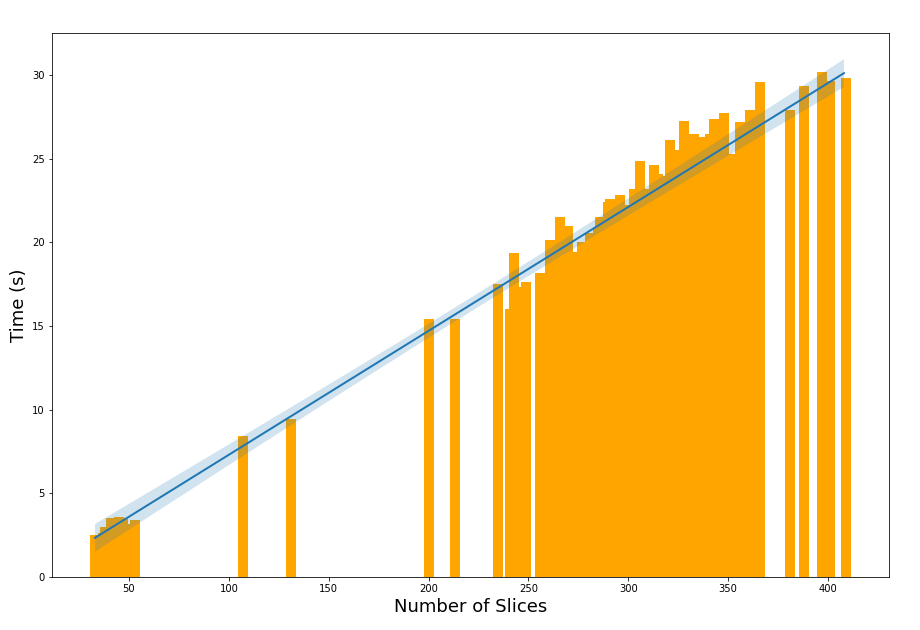
\includegraphics[scale=.75]{Timing_lab.png}
		\caption{Total labeling time vs number of slice for each scan of each dataset}	\label{fig:Timing_lab}
		
	\end{figure}
	
\end{document}

